\section{Opérateurs de flux}\label{sec:contrib:astral:flux}
Astral repose sur deux concepts. Ainsi, il est nécessaire définir les opérateurs de flux vers relation (fenêtres) et de relation vers flux (streamers). Puis, nous définissons des opérateurs spécifiques : la gestion des modifications des relations temporelles et des \textit{batchs}.
\subsection{Fenêtres}
Comme nous l'avons vu dans la section~\ref{sec:rw:sgfd:modeles}, l'opérateur de fenêtre est un des opérateurs les plus étudiés dans la littérature. Toutefois, son comportement est encore flou sur certains points. La formalisation de son fonctionnement permet une meilleure spécification.
\subsubsection{Association position-\textit{batch}}
Avant de définir formellement l'opération de fenêtrage, nous avons besoin d'un outil pour gérer l'association entre la position d'un n-uplet et de son \textit{batch}. La fonction $\tau_S$ définit cette association (def~\ref{def:tau}). 
\begin{defi}[Fonction position-\textit{batch}]\label{def:tau}
    Soit $S$ un flux,

    La fonction $\tau_S : \N\to \TN$ est la fonction qui par une position (dans $\N$) donne l'identifiant du batch (dans $\TN$) du seul n-uplet ayant cette position.

    Par convention, $\tau_S(0)=(t_0,0)$.
\end{defi}

En corollaire de l'hypothèse des ordres~\ref{hyp:ordres}, la fonction $\tau_S$ est croissante non-stricte. Ainsi, il est possible de définir une pseudo inverse (cor~\ref{cor:rtau}) $\rtau_S$ capable de donner une position (la maximale) pour un \textit{batch} donné.
\begin{coro}[Fonction pseudo-inverse de $\tau$]\label{cor:rtau}
    Soit $S$ un flux,

    La pseudo-inverse $\rtau_S:\TN\to \N$ existe et correspond à la plus grande position du \textit{batch} donné en entrée. Si aucun \textit{batch} n'existe, le plus proche est utilisé. Formellement, $$\forall b \in \TN, \qquad \tau_S^{-1}(b) = \sum_{n=0}^{+\infty} n \indic_{[\tau_S(n),\tau_S(n+1)[}(b)$$
\end{coro}

\subsubsection{Description de séquences de fenêtres}
Afin de se rapprocher le plus possible d'un aspect déclaratif, il est nécessaire de décomposer l'opérateur de fenêtre en deux objets mathématiques : la description de son évolution et la séquence de fenêtres. Cette dernière prend une description en argument pour représenter la relation temporelle résultante. Le principe des descriptions de séquences de fenêtres tel que décrit dans la définition~\ref{def:dsf}) est assez simple puisqu'il suffit de décrire deux bornes ($\alpha$ et $\beta$) évoluant de manière discrète ainsi qu'un taux d'évaluation de ces bornes ($r$).

\begin{defi}[Description de Séquence de Fenêtre (DSF)]\label{def:dsf}
    Soient $\D$ et $\D'$ pouvant être $\T$ ou $\N$, une description de séquence de fenêtre (DSF) est un triplet $(\alpha,\beta,r)$ tel que :
\begin{itemize}
    \item $r \in \D$ est le taux d'évaluation des bornes de la fenêtre
    \item $\alpha$ et $\beta$ sont deux fonctions de $\N\to D'$ représentant l'évolution des bornes.
\end{itemize}

$\alpha(j)$ et $\beta(j)$ définissent les $j\eme$ valeurs des bornes. La première borne est donnée pour $j=0$. Ces fonctions se doivent de vérifier les propriétés suivantes (en considérant $\D=\D'=\T$) :
$$\forall j \in \N, \begin{cases} \alpha(j) \leq \beta(j) & \textrm{le début est avant la fin}\\ \alpha(j) \geq t_0 & \textrm{le début existe} \\ \beta(j) \leq jr + \beta(0) & \textrm{la fin est accessible} \end{cases}$$
    Les conditions pour les autres cas pour $\D$ et $\D'$ se déduisent par application des fonctions $\tau_S$ et $\rtau_S$.
\end{defi}

\begin{example}
    Nous souhaitons connaître tous les $100$ relevés de charge processeur, les $10$ derniers relevés. Dans ce cas, nous souhaitons obtenir une séquence de fenêtres positionnelles générées tous les $100$ n-uplets ($r=100\in \N$). Nous appliquons des bornes positionnelles $\alpha,\beta \in (\N\to\N)^2$. La première fenêtre contient du $91\eme$ n-uplet au $100\eme$. Ainsi : $\alpha(0) = 91$ et $\beta(0) = 100$. Sachant que l'évolution des bornes est linéaire, nous avons :
\begin{eqnarray*}
 \alpha(j) &=& 100j+91\\
 \beta(j) &=& 100j + 100\\
 r & = & 100
\end{eqnarray*}
\end{example}

La création de fenêtres nécessite d'associer les n-uplets du flux et le numéro de fenêtre décrit dans la \textit{DSF}. Pour cela, nous définissons en~\ref{def:gamma} une \textit{fonction d'attente} utilisant les identifiants de \textit{batchs}. Cette fonction donne le rang de la dernière fenêtre complète au moment du batch. Le terme \textit{attente} est lié au fait que l'évaluateur de fenêtre doit attendre le prochain changement de $\gamma$.
Nous retrouvons dans cette fonction le caractère \textit{bloquant} des fenêtres.
\begin{defi}[Fonction d'attente $\gamma$]\label{def:gamma}
    Soit $S$ un flux, soit $(\alpha,\beta,r)$ une DSF,

    La fonction d'attente de la DSF est une fonction $\TN \to \N$ permettant de trouver pour un identifiant de \textit{batch}, l'identifiant de la dernière fenêtre complétée.
\begin{itemize}
 \item  Si $r\in\T$, cette fonction est définie par $\gamma : (t,i) \mapsto \left\lfloor \frac{t-\beta(0)}{r} \right\rfloor$.
 \item  Si $r\in\N$, cette fonction est définie par $\gamma : (t,i) \mapsto \left\lfloor \frac{\rtau_S(t,i)-\beta(0)}{r} \right\rfloor$.
\end{itemize}
\end{defi}
\begin{example}
    En reprenant l'exemple précédent, après simplification nous obtenons : $$\gamma(b) = \left\lfloor \frac{\rtau_S(b)}{100}\right\rfloor-1.$$
    Si nous supposons que le flux produit un n-uplet par seconde (ainsi, $\rtau_S(t,i) = \lfloor t/1s \rfloor$) : alors $\gamma(1024s,0) = \left\lfloor \frac{1024}{100}\right\rfloor-1 = 9$. Nous avons bien la $10\eme$ fenêtre ($j=9$) comme la dernière fenêtre créée à l'instant 1024.
\end{example}

\subsubsection{L'opérateur}
Il devient désormais possible de définir un opérateur permettant de générer une relation temporelle à partir d'un flux donné. Cette relation temporelle change d'état avec l'instant défini par la fonction $\gamma$. De manière générale, une DSF peut être ramenée à une expression plus générale $(\alpha,\beta,\gamma)$ ce que nous utilisons pour la définition~\ref{def:fenetre} de séquence de fenêtres.
\begin{defi}[Opérateur de Séquence de Fenêtres]\label{def:fenetre}
	Soit $S$ un flux et $(\alpha, \beta, \gamma)$ une description de séquence,
	
	L'opérateur de séquence de fenêtres est défini par : $\forall b \in \TN$, 
	\begin{itemize}
		\item Si $\gamma(b) \geq 0$, 
		\begin{itemize}
			\item Si la description possède des bornes temporelles :
			$$S[\alpha,\beta,\gamma](b) = \left\{s\in S, \ (\alpha(\gamma(b)),0)\leq \BS(s) \leq (\beta(\gamma(b)),i)\right\}$$
			\item Si la description possède des bornes positions :
			$$E(b) = \left\{s\in S, \ \tau_S(\alpha(\gamma(b)))\leq \BS(s) \leq \tau_S(\beta(\gamma(b)))\right\}$$
			$$S[\alpha,\beta,\gamma](b) = \{s \in E(b) / (\#E(b) - \pos_{E(b)}(s)) \leq \beta(\gamma(b)) - \alpha(\gamma(b))$$
		\end{itemize}
		\item Si $\gamma(b) <0$ alors $S[\alpha,\beta,\gamma](b) = \emptyset$
	\end{itemize}
\end{defi}

Plusieurs remarques peuvent être formulées sur cette définition. Tout d'abord, les expressions sont différentes si les bornes sont positionnelles ou temporelles. Pour les fenêtres temporelles, l'opérateur inclut les n-uplets dont l'identifiant de \textit{batch} s'étend :
\begin{itemize}
	\item[\textbf{depuis}] le premier \textit{batch} de la fenêtre : $(\alpha(\gamma(t,i)),0)$, i.e. ceux dont le \textit{timestamp} est supérieur à la borne inférieure.
	\item[\textbf{jusqu'au}] dernier \textit{batch} de la fenêtre : $(\beta(\gamma(t,i)),i)$. Ce qui correspond au $i\eme$ \textit{batch} ayant le \textit{timestamp} inférieur ou égal à la borne.
\end{itemize}
Il est important de voir que $S[\alpha,\beta,\gamma]$ peut changer à l'arrivée d'un nouveau \textit{batch}, même si le \textit{timestamp} ne change pas. Ne pas inclure ces modifications ferait perdre des données à la fenêtre. Nous retrouvons les problématiques explorées dans la section~\ref{sec:rw:sgfd:modeles}.

Pour les fenêtres positionnelles, la gestion est plus délicate. Si nous considérons que le flux réparti ses \textit{batchs} (un n-uplet par \textit{batch}), alors $E(b) = S[\alpha,\beta,\gamma](b)$. Mais dans le cadre général, $E(b)$ contient l'ensemble des n-uplets potentiels et la séquence $S[\alpha,\beta,\gamma](b)$ en est un sous-ensemble dont la taille est exactement celle décrite dans la DSF (sélections des n-uplets les plus récents). De plus, nous remarquons que $\gamma$ en positionnel est défini en fonction de $\rtau_S$ qui fournit la position maximale en cas d'égalité de \textit{batchs}, ce qui nous garanti de couvrir l'ensemble des n-uplets concernés.


\begin{example}
	La figure~\ref{fig:contrib:astral:fenetres} montre l'évolution d'une séquence où la fenêtre glisse de $2$ secondes toutes les $2$ secondes ($r=2$) avec une taille constante de $3$ secondes. $t_0 = 0$ par simplicité ici. 
La première fenêtre possède les bornes $\alpha(0) = t_0+ 0s$ et $\beta(0) =t_0+3s$. Sachant que le glissement est de $2s$ la description de fenêtre est $$\forall j \in \N, \begin{cases} \alpha(j)  & =\ j*2s+t_0 \\ \beta(j) & = \ j*2s+3s+t_0\end{cases}$$
La relation temporelle générée par cette DSF peut être notée $S[2js,2js+3s,2s]$.  Le calcul de son état à un instant est simple. Prenons le \textit{batch} $(t_0+5.5s,0)$. La fenêtre à calculer est la fenêtre numérotée $\gamma(t_0+5.5s,0) = \left\lfloor \frac{t_0+5.5s-\beta(0)}{r}\right\rfloor = 1$. Ainsi : $S[2js,2js+3s,2s](t_0+5.5s,0) = F_1 = \{s_4,s_5,s_6,s_7,s_8\}$.
\end{example}
\begin{figure}[ht]
	\centering
	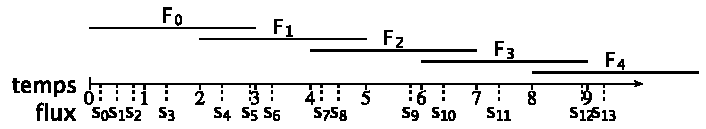
\includegraphics[width=0.7\textwidth]{contrib-astral-fenetres}
	\caption{Séquence de fenêtre de taille $3s$ glissante de $2s$}\label{fig:contrib:astral:fenetres}
\end{figure}

\begin{defi}[Exclusions de bornes de fenêtres]\label{def:exclufenetre}
    Soit $S$ un flux et $(\alpha,\beta,\gamma)$ une description de séquence de fenêtre,

    Les notations $S]\alpha,\beta,\gamma]$, $S[\alpha,\beta,\gamma[$ et $S]\alpha,\beta,\gamma[$ désignent les définitions de l'opérateur classique de séquence de fenêtre permettant d'exclure respectivement les bornes inférieures, supérieures ou les deux.
\end{defi}

\begin{example}
    En reprenant la définition de fenêtre sur 5 secondes : $(j*5s+t_0,j*5s+5s+t_0,5s)$. Nous remarquons que les fenêtres 0 et 1 contiennent les n-uplets dont le \textit{timestamp} est égal à $t_0+5s$. Ainsi, l'opérateur $S]jr+t_0,jr+r+t_0,r]$ avec $r=5s$ permet de retirer les n-uplets à ce \textit{timestamp} de cette fenêtre.
\end{example}

\subsubsection{Fenêtres partitionnées}
L'opérateur de fenêtres partitionnées est très utilisé pour appliquer la même séquence de fenêtres à des sous-flux. Les opérateurs partitionnés sont tous décrits de la même manière. Le principe, illustré dans la figure~\ref{fig:contrib:astral:partition} est de diviser le flux suivant un (ou des) attribut $A$ donné. Sur chacun de ces sous-flux est appliqué un opérateur quelconque. Le résultat est l'union des résultats de ces opérateurs.

\begin{figure}[ht]
	\centering
	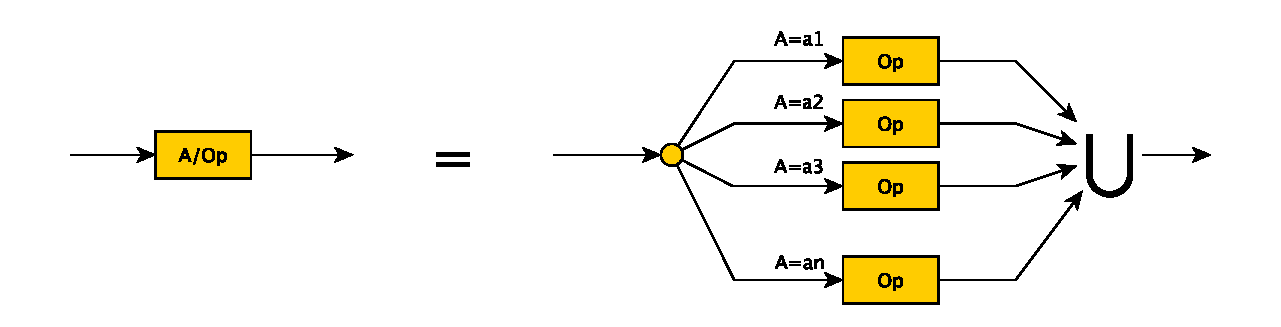
\includegraphics[width=0.9\textwidth]{contrib-astral-partition}
	\caption{Principe d'un opérateur partitionné}\label{fig:contrib:astral:partition}
\end{figure}

Ainsi, nous décrivons dans la définition~\ref{def:partition} de séquence de fenêtre partitionnée l'application de ces principes de partitionnement sur l'opérateur de séquence de fenêtre.
\begin{defi}[Séquence de fenêtre partitionnée]\label{def:partition}
	Soient $S$ un flux, $a_1,...,a_k$ un ensemble d'attributs du schéma de $S$, et $(\alpha,\beta,\gamma)$ une DSF,
	
	Soit $\cup^*$ l'union relationnelle conservant les identifiants physiques, 

	Alors, la séquence de fenêtres $(\alpha,\beta,\gamma)$ partitionnées par $a_1,...,a_k$ est définie par :
	$$S[a_1...a_k/\alpha,\beta,\gamma] = \mathop{\bigcup\null^*}_{a\in Dom(a_1,...,a_k)} (\sigma_{(a_1,...,a_k)=a} S)[\alpha,\beta,\gamma]$$
\end{defi}

Nous remarquons que nous utilisons la définition de l'union relationnelle conservant les identifiants physiques présentés dans la section précédente, ainsi l'ordre naturel décrit dans le flux d'entrée peut être retrouvé dans la relation de sortie.
\begin{example}
	L'exemple le plus courant est la représentation de l'état actuel d'un système à partir d'un flux. Supposons un flux d'entrée $CPU(appId,cpu,\t)$, nous donnant les relevés de charge de processeur. Soit la description de fenêtre rapportant le dernier n-uplet d'un flux : $(1j,1j,1)$. Nous pouvons obtenir la relation temporelle représentant pour chaque application $appId$, la dernière valeur connue de $cpu$ ainsi que le \textit{timestamp $\t$ de mesure} : $$CPU[appId/1j,1j,1]$$

	Cet exemple illustre comment nous pouvons passer d'un flux brut à une représentation (dynamique) d'un \textbf{contexte}. 
	
	La définition du partitionnement par l'union conservant les identifiants physiques permet d'avoir un ordre clair et intuitif sur la relation temporelle résultante. Lorsqu'un nouveau n-uplet entre dans cette relation (ou remplace l'ancien n-uplet), alors il est mis en bout. Avec l'union classique, il est nécessaire de définir l'ordre d'application des unions. Et les n-uplets auraient changé d'identifiants à chaque nouvel état de la fenêtre, ce qui est difficile à contrôler et à manipuler.
\end{example}

Par la suite, plusieurs notations simplifiées sont utilisées pour désigner des descriptions de fenêtres courantes décrites dans le tableau~\ref{tab:windows}.
\begin{table}[ht]
\centering
\begin{tabular}{c||p{0.4\textwidth}|p{0.4\textwidth}}
  & Définition & Équivalence \\ \bottomrule
 $[L]$ & $[j,j,1]$ &  \\ 
 & \multicolumn{2}{p{0.8\textwidth}}{La séquence de fenêtre où chaque fenêtre ne contient que le dernier n-uplet du flux. Cette séquence est égale à $[B]$ si le flux répartit ses n-uplets avec un n-uplet par \textit{batch}.} \\ \hline
 $[B]$ & $]\tau_S^{-1}(\tau_S(j)^-),j,1]$ & $\{s\in S, \BS(s) = \tau_S\circ\tau_S^{-1}(b)\}$ \\ 
 & \multicolumn{2}{p{0.8\textwidth}}{Séquence de fenêtre où chaque fenêtre contient le dernier \textit{batch}.} \\\hline
 $[\infty]$ & $[0,j,1]$ & $\{s\in S, \BS(s) \leq b\}$ \\
 & \multicolumn{2}{p{0.8\textwidth}}{Séquence cumulative contenant tout le flux jusqu'au \textit{batch} courant.} \\\hline
 $[T\ r\ s]$ & $]\max(sj-r+t_0,t_0),sj+t_0,s]$ &  \\
 & \multicolumn{2}{p{0.8\textwidth}}{Fenêtre temporelle de taille $r$ se déplaçant toutes les $s$ unités de temps.} \\\hline
 $[P\ r\ s]$ & $]\max(sj-r,0),sj,r]$ &  \\
 & \multicolumn{2}{p{0.8\textwidth}}{Fenêtre positionnelle de taille $r$ n-uplets se déplaçant tous les $s$ n-uplets.} \\
 \toprule
\end{tabular}
\caption{Liste des fenêtres courantes} \label{tab:windows}
\end{table}
Il est important de noter que les équivalences citées sont non triviales, des démonstrations formelles sont fournies en annexes~\ref{misc:fenetres}.

\subsection{Streamers}
La classe des \textit{streamers} est l'ensemble des opérateurs produisant un flux à partir d'une relation. Son utilisation, après l'application d'une fenêtre, permet la création d'un flux résultant. La définition des streamers est découpée en deux parties, d'abord la définition de la réécriture de \textit{timestamp} qui permet d'ajouter le \textit{timestamp} aux données produites, et ensuite la définition de l'opérateur.
\subsubsection{Réécriture de \textit{timestamp}}
Il est nécessaire de gérer les identifiants physiques. En effet, si un n-uplet est envoyé plusieurs fois dans le flux résultat, il y a conflit si $\varphi$ n'est pas modifié. De plus, tout flux doit avoir un attribut $\t$. Cet attribut doit être créé ou remplacé pour assurer l'hypothèse des ordres. Le principe est que le n-uplet $s\in R(b)$ doit être envoyé dans le flux au \textit{batch} $(t_s,i_s)$, alors nous devons envoyer le n-uplet $\Psi_b(s,t_s)$ décrit dans la définition~\ref{def:stamping}.
\begin{defi}[Fonction de réécriture de \textit{timestamp}]\label{def:stamping}
    Soit $R$ une relation de schéma $A$, $b$ un batch,

    Soit $\I^S = \TN\times \I_R$ le $\Phi$-espace ordonné de manière naturelle,

    La fonction de réécriture de \textit{timestamp} appliquée à $R(b)$ est définie par : 
$$\forall s\in R(b), \ \forall t_s\in\T, \ \Psi_b(s,t_s) = \{(\t,t_s), (\varphi, (b,s(\varphi)))\}\bigcup_{a\in A\backslash\{\varphi,\t\}}\{(a,s(a))\}$$
\end{defi}

Cette définition assure que les nouveaux n-uplets du flux vérifient les propriétés suivantes : 
\begin{itemize}
 \item Ils ont pour \textit{timestamp} $t_s$ le moment où il a été estampillé.
 \item Ils ont un identifiant physique (et du coup une position) plus grand que les identifiants précédents.
 \item L'ordre positionnel de $R(b)$ est préservé.
\end{itemize}
Nous pouvons définir des \textit{streamers} dit sensibles dans la définition~\ref{def:streamers}). Ces \textit{streamers} réagissent aux changements de $R$ et produisent un flux en conséquence.
\begin{defi}[\textit{Streamers} sensibles]\label{def:streamers}
    Soit $R$ une relation,

    Les \textit{streamers} sensibles sont les opérateurs créateurs d'un flux $S$ défini à partir des changements de $R$, trois types sont définis :
\begin{itemize}
 \item Le \textit{streamer} d'insertion, envoyant les nouveaux n-uplets : $\IS(R)$, $$s\in R(t,i) \wedge s\not\in R((t,i)^-) \equ s'=\Psi_{(t,i)}(s,t)\in S \wedge \BS(s') = (t,i)$$
 \item Le \textit{streamer} de suppression, envoyant les n-uplets disparus : $\DS(R)$, $$s\not\in R(t,i) \wedge s\in R((t,i)^-) \equ s'=\Psi_{(t,i)^-}(s,t)\in S \wedge \BS(s') = (t,i)$$
 \item Le \textit{streamer} d'envoi, envoyant tous les n-uplets présents : $\RSu(R)$, $$s\in R(t,i) \neq R((t,i)^-) \equ s'=\Psi_{(t,i)}(s,t)\in S \wedge \BS(s') = (t,i)$$
\end{itemize}
\end{defi}

Nous avons constitué la chaîne complète permettant de traiter les flux de données : flux vers relation, relation vers relation, et relation vers flux. Nous allons explorer un exemple complet pour montrer la clarté d'expression issue de l'algèbre.

\begin{example}
    Le flux d'alerte avec pour attributs (deviceId, avgcpu, $\t$) représente que l'équipement \textbf{deviceId} au \textit{timestamp} $\t$ a eu une charge moyenne \textit{avgcpu} supérieure à 25\%. La moyenne est calculée sur 5 min toutes les minutes.

    Pour former ce flux, il est nécessaire de joindre le flux \textbf{CPU} avec \textbf{Applications} afin de pouvoir associer le bon \textit{deviceId} à l'\textit{appId}. Or, cette opération est interdite à moins de faire une fenêtre sur le flux. Nous pourrions utiliser une fenêtre telle que le dernier \textit{batch} $[B]$, mais comme il est nécessaire d'obtenir une fenêtre temporelle pour le calcul de moyenne, nous pouvons appliquer la description appropriée : $$CPU[T\ 5min\ 1min]\Join Applications.$$

    Appliquons l'opération d'agrégation sur cette relation pour obtenir la moyenne. Puis nous pouvons sélectionner les n-uplets la moyenne est supérieure à 25\%. Enfin, le flux doit être créé à partir de la relation temporelle représentant les équipements supérieurs à 25\% de charge pendant les 5 dernières minutes. Ici une ambiguïté réside dans l'énoncé. Souhaitons-nous avoir le flux des nouveaux équipements ayant ce problème ou souhaitons-nous être notifiés à chaque vérification ? Ce critère va influencer le choix du \textit{streamer} : $\IS$ ou $\RSu$. Prenons le premier, nous obtenons la requête suivante : 
    $$\IS\left(\sigma_{avgcpu \geq 25} \ \null_{deviceId}\G_{avg_{cpu}^{avgcpu}} (CPU[T\ 5min\ 1min]\Join Applications)\right)$$
\end{example}

D'autres streamers peuvent être construits pour effectuer l'insertion de données dans le flux résultat de manière périodique comme le présente la définition~\ref{def:rsr}.
\begin{defi}[\textit{Streamers} périodiques]\label{def:rsr}
    Soit $R$ une relation,

    Les \textit{streamers} périodiques sont les opérateurs créateurs d'un flux $S$ où les insertions ont lieu périodiquement. Le \textit{streamer} $\RS{r}$ est défini par un taux temporel $r$ et la propriété :
$$s\in R(t,i) \wedge t-t_0\equiv 0[r]\equ s'=\Psi_{(t,i)}(s,t)\in S \wedge \BS(s') = (t,i)$$
\end{defi}

Nous avons maintenant défini des opérateurs permettant de couvrir la plupart des opérations. Toutefois, deux opérateurs sont encore à définir pour certaines opérations plus particulière.
\subsection{Manipulation temporelle}\label{sec:contrib:astral:manipulation}
Contrairement à l'algèbre relationnelle, les relations sont temporelles ici. Elles changent au cours de l'exécution de la requête. Il n'existe pas d'opérateurs capables de contrôler ces changements. L'opérateur de manipulation temporelle permet de sélectionner, pour l'instant présent, un état passé d'une relation. Tout d'abord, définissons une transformation temporelle avec la définition~\ref{def:transformation} permettant de sélectionner l'instant voulu sur la relation temporelle. La seule contrainte de cette transformation est l'impossibilité de regarder dans le futur. Nous pouvons ainsi définir l'opérateur de manipulation temporelle (def~\ref{def:manipulation}) qui applique cette transformation à la relation temporelle.
\begin{defi}[Transformation temporelle]\label{def:transformation}
    Une transformation temporelle est une fonction de $\TN\to\TN$ telle que $\forall b\in\TN, f(b) \leq b$.
\end{defi}

\begin{defi}[Opérateur de manipulation temporelle]\label{def:manipulation}
    Soient $R$ une relation, $c$ une condition sur $\TN$ et $f$ une transformation temporelle,

    Alors l'opérateur de manipulation temporelle est défini par $$\D_c^f(R) = b \mapsto \begin{cases} R(f(b)) & \textrm{ si } c(b) \\ \emptyset & \textrm{ sinon}\end{cases}$$
\end{defi}

Plusieurs fonctions classiques ont une utilité directe :
\begin{itemize}
 \item $\mathrm{freeze}^{t_s}(t,i)=(t_s,0)$ si $t \geq t_s$. Permet de figer une relation temporelle à un instant précis, plus aucun changement n'est retransmis à partir de ce point. La relation résultante de cette opération est notée $R^{t_s}$. Un cas particulier est lorsque $t_s=t_0$. Dans ce cas la relation n'a qu'un seul état. Grâce à cette opération, nous sommes capables de faire une \textbf{interrogation instantanée} sur des relations temporelles.
 \item $\mathrm{period}^r(t,i)=\left(\left\lfloor\frac{t-t_0}{r}\right\rfloor r + t_0, 0\right)$ met à jour la relation de manière périodique avec un taux de rafraîchissement $r$.
 \item $\mathrm{change}_S(t,i)=\tau_S\circ\rtau_S$ met à jour la relation à chaque fois qu'un \textit{batch} est inséré dans $S$. Le même principe permet une mise à jour \textit{à chaque fois que la relation $R'$ change}.
\end{itemize}

Cette dernière fonction a un impact particulier lors de la jointure de deux relations temporelles. Dans la jointure (ou au sens large le produit cartésien) telle que nous l'avons définie, si un changement est appliqué d'un côté ou de l'autre, un nouveau calcul de jointure est effectué. Ce comportement peut ne pas être souhaité dans la pratique où nous pourrions souhaiter que seule une branche soit déclencheur de calcul et l'autre soit passive. La jointure semi-sensible permet cette opération. Dans la définition~\ref{def:ssjoin} le résultat $R_1 \ssjoin R_2$ n'est pas mis à jour au changement de $R_2$ mais au changement de $R_1$ avec l'état de $R_2$ correspondant.

\begin{defi}[Jointure semi-sensible]\label{def:ssjoin}
    Soient $R_1$ et $R_2$ deux relations temporelles,

    Soit $\mathrm{change}_{R_1}$ la transformation temporelle telle que $\mathrm{change}_{R_1}(b)$ correspond au dernier changement de $R_1$ inférieur ou égal à $b$,

    La jointure semi-sensible est définie par :
        $$R_1\ssjoin R_2 = R_1 \Join \D^{\mathrm{change}_{R_1}}(R_2)$$
\end{defi}
\begin{example}
    $$DeviceCPU=\IS(\Pi_{deviceId,deviceName,cpu}(CPU[B]\Join Applications)\ssjoin Devices)$$

Le flux résultat $DeviceCPU$ correspond au flux \textit{CPU} originel sur lequel nous avons remplacé l'attribut \textit{appId} par les attributs \textit{deviceId} et \textit{deviceName} qui sont plus intéressants d'un point de vue de l'observation. Si \textit{Devices} est mise à jour (pour changer son statut) en utilisant la jointure simple, la relation temporelle change d'état. Ce qui provoque l'envoi d'un nouveau n-uplet dans le flux. L'opérateur de jointure semi-sensible empêche ce cas puisque les mises à jour sont cadencées par celles de $CPU[B]\Join Applications$ c'est-à-dire $CPU[B]$ soit encore les \textit{batchs} de $CPU$ et non la relation \textit{Devices}.
\end{example}

\subsection{Spread}
Enfin, le dernier opérateur est celui évoqué lors de la conception des \textit{batchs} dans~\cite{Jain:spread}. Il est nécessaire d'avoir un opérateur pour manipuler les \textit{batchs} afin de modifier la fonction $\BS$ d'un flux sans toucher à ses données.

L'opérateur de réinitialisation des \textit{batchs} (def~\ref{def:spreadall}, \textit{spread all} dans la littérature) permet de rassembler les \textit{batchs} multiples pour chaque \textit{timestamp} en un seul. Ceci permet de réorganiser le flux.
\begin{defi}[Réinitialisation des batch]\label{def:spreadall}
Soit $S$ un flux,

Le flux $S$ réinitialisé noté $\lhd S$ vérifie :
$$\forall s\in S, \textrm{ alors } s \in \lhd S, \textrm{ et }\B{\lhd S}(s) = (s(\tau),0)$$
\end{defi}

L'opérateur \textit{spread} décrit dans la définition~\ref{def:spread} permet de découper les \textit{batchs} présents dans un flux en plusieurs nouveaux. Le découpage se fait sur l'ordre induit par ses attributs. Ceci permet par exemple de partitionner selon un identifiant.
\begin{defi}[\textit{Spread}]\label{def:spread}
Soient $S$ un flux de schéma $A$, et $a$ un attribut de $S$,

Soit $\I^S = \TN\times \I_R$ le $\Phi$-espace ordonné de manière lexicographique,

Alors le flux $S$ raffiné par l'attribut $a$ noté $\rhd_{a} S$ vérifie :
$\forall s_1, s_2\in S^2, \textrm{ alors } s_1', s_2' \in (\rhd_a S)^2,$ tel que :
\begin{eqnarray*}
b_1=\B{\rhd_a S}(s_1') < b_2=\B{\rhd_a S}(s_2') &\equ & \BS (s_1) < \BS (s_2)\\ & & \quad \vee \ \left(\BS (s_1) = \BS (s_2)\right. \\ & & \quad\quad \quad\quad\wedge \ \left.s_1(a) < s_2(a)\right)
\end{eqnarray*}

Ainsi que $s_i' = \{(\varphi, (b_i,s_i(\varphi)))\}\bigcup_{x\in A\backslash\{\varphi\}}\{(x,s(x))\}$, pour $i\in\{1,2\}$
\end{defi}

Originellement, si pour l'opérateur \textit{spread}, aucun attribut n'est mentionné, alors tous les n-uplets sont étalés dans des batchs séparés de manière non déterministe. Dans notre algèbre, l'attribut $\varphi$ et l'ordre positionnel permettent de définir l'ordre des \textit{batchs} comme l'ordre positionnel : $\rhd = \rhd_\varphi$. À l'inverse, en appliquant $\lhd$, nous définissons l'ordre des \textit{batchs} comme l'ordre temporel.

\begin{example}
Sachant le contenu du flux \textbf{CPU}(appId, value, $\t$) :

\begin{center}\noindent\begin{tabular}{|c|c|c|} \bottomrule
(1,0) & (1,1) & (2,0) \\ \hline
\begin{tabular}{c}
$(1,20,1)$ \\
$(1,25,1)$ \\
$(2,22,1)$ \\
\end{tabular} &
\begin{tabular}{c}
$(4,10,1)$ \\
$(1,25,1)$ \\
$(4,12,1)$ \\
\end{tabular} &
\begin{tabular}{c}
$(2,23,1)$ \\
$(6,64,1)$ \\
\end{tabular} \\ \toprule
\end{tabular}
\end{center}

 $\lhd\ CPU$ : L'application de l'opérateur de réinitialisation des \textit{batchs} regroupe tous les n-uplets simultanés dans le même \textit{batch}.
 
\begin{center}\noindent\begin{tabular}{|c|c|} \bottomrule
(1,0) & (2,0) \\ \hline
\begin{tabular}{c}
$(1,20,1)$ \\
$(1,25,1)$ \\
$(2,22,1)$ \\
$(4,10,1)$ \\
$(1,25,1)$ \\
$(4,12,1)$ \\
\end{tabular} &
\begin{tabular}{c}
$(2,23,1)$ \\
$(6,64,1)$ \\
\end{tabular} \\ \toprule
\end{tabular}
\end{center}

 $\rhd_{appId}\ CPU$ : L'utilisation du \textit{spread} sur l'identifiant permet d'affiner les \textit{batchs} originels en garantissant que chaque \textit{batch} ne contienne qu'une valeur de \textit{appId}.
 
\begin{center}\noindent\begin{tabular}{|c|c|c|c|c|c|} \bottomrule
(1,0) & (1,1) & (1,2) & (1,3) & (2,0) & (2,1) \\ \hline
\begin{tabular}{c}
$(1,20,1)$ \\
$(1,25,1)$ \\
\end{tabular} &
\begin{tabular}{c}
$(2,22,1)$ \\
\end{tabular} &
\begin{tabular}{c}
$(1,25,1)$ \\
\end{tabular} &
\begin{tabular}{c}
$(4,10,1)$ \\
$(4,12,1)$ \\
\end{tabular} &
\begin{tabular}{c}
$(2,23,1)$ \\
\end{tabular} &
\begin{tabular}{c}
$(6,64,1)$ \\
\end{tabular} \\ \toprule
\end{tabular}
\end{center}

$\lhd\rhd_{appId}\ CPU$ : La combinaison de la réinitialisation et du \textit{spread} permettent d'avoir un \textit{batch} par \textit{timestamp} affecté à une valeur d'\textit{appId}.

\begin{center}\noindent\begin{tabular}{|c|c|c|c|c|} \bottomrule
(1,0) & (1,1) & (1,2) & (2,0) & (2,1) \\ \hline
\begin{tabular}{c}
$(1,20,1)$ \\
$(1,25,1)$ \\
$(1,25,1)$ \\
\end{tabular} &
\begin{tabular}{c}
$(2,22,1)$ \\
\end{tabular} &
\begin{tabular}{c}
$(4,10,1)$ \\
$(4,12,1)$ \\
\end{tabular} &
\begin{tabular}{c}
$(2,23,1)$ \\
\end{tabular} &
\begin{tabular}{c}
$(6,64,1)$ \\
\end{tabular} \\ \toprule
\end{tabular}
\end{center}
\end{example}

Nous avons maintenant présenté l'ensemble des opérateurs de l'algèbre Astral. Nous sommes désormais capables d'exprimer une requête continue (et instantané avec l'aide de la manipulation temporelle) avec une grande clarté et sans ambiguïté sémantique. Nous allons maintenant, définir l'équivalence de requête avec des \textit{timestamps} de départs $t_0$ différents.